\chapter{Probing Lightning channel balances}

\label{Chapter06LNprobing}

The LN protocol provides no way for a node to know how funds are split in remote channels.
But how private is this information in practice?
In this Chapter, we show that a low-resource attacker can infer balances of most of the channels.\footnote{This Chapter is based on~\cite{Tikhomirov2020}.}
We describe an algorithm that reveals channel balances using \textit{probing} -- sending a fake payment (a \textit{probe}) and observing the resulting error.
Our method shows better accuracy and cost compared to similar approaches described in the literature.
Our technique scales to the whole network and achieves high precision.
It requires moderate capital commitment, half of the channels can be probed in $21$~seconds.
The attacker's capital is not spent, but only temporarily locked up.
Compared to earlier approaches~\cite{HerreraJoancomarti2019, Dam2019}, we can probe \textit{remote} channels (i.e.,~without establishing a channel with one of their endpoints).
This greatly reduces time and capital required for the attack.
We test our proof-of-concept implementation on Bitcoin testnet and successfully probe a significant portion of its channels.
We also outline potential countermeasures, which include changes in error handling, sharing channel balances explicitly, and \textit{just-in-time} (JIT) routing.

On a more general note, we raise a question of the \textit{privacy-efficiency trade-off} in the LN\@.
At the moment, LN nodes cannot use balance information for routing, which leads to failed payments, but balances are extractable by an attacker anyway.
Can we strike a better balance between balance privacy and routing efficiency?
Answering this question remains an exciting avenue for future work.


\section{Probing algorithm}
\label{sec:probing}

\subsection{Overview}

As described in Chapter~\ref{Chapter05IntroLightning}, a payment channel operates as follows.
Two parties lock funds in a multi-signature transaction output and then change the distribution of funds in a sequence of nearly instant off-chain transactions.
LN nodes gossip about channels available for routing and their total capacities.
To issue a multi-hop payment, the sender creates a route based on its local knowledge of the network.
The current channel balances are not announced.

Consider two LN nodes that share a channel.
Let us denote the total capacity of the channel as $c$.
LN channels are bidirectional.
Without loss of generality, let us denote one of the nodes as \textit{source} (with balance $b_s$) and the other as \textit{destination} (with balance $b_d$).\footnote{As per BOLT specification, the source is defined as the node with an alphanumerically smaller node ID.}
By definition, $c = b_s + b_d$.
Our goal is to determine how $c$~is split between $b_s$~and~$b_d$.
For concreteness, for each channel, we estimate $b_s$, and refer to it simply as $b$.

In a nutshell, our algorithm consists of the following steps:
\begin{itemize}
	\item set up a Lightning node;
	\item open a few \textit{entry channels} to manually selected nodes (\textit{entry nodes});
	\item compile the list of channels for probing;
	\item for each channel in the list, do a binary search for the value of~$b$~by sending fake payments through routes ending with the chosen channel.
\end{itemize}

\subsection{Assumptions}

To be suitable for probing, the channel must be \textit{active} (available for routing) and \textit{live} (responding to requests).
We assume that nodes follow the BOLT specification (in particular, they return errors as prescribed).

\paragraph{Error interpretation}
Our method uses two types of errors, which have a broader semantics than our method is aware of.
\texttt{temporary\_channel\_failure} (\texttt{UPDATE|7}) is returned if a forwarding node "was unable to handle this HTLC, but may be able to handle it, or others, later".
We interpret this error as "insufficient balance", though there may be other reasons for a channel to be temporarily unavailable.
\texttt{incorrect\_or\_unknown\_payment\_details} (\texttt{PERM|15}) is returned if "[t]he payment\_hash is unknown to the final node, the payment\_secret doesn't match the payment\_hash, the amount for that payment\_hash is incorrect or the CLTV expiry of the HTLC is too close to the current block height for safe handling".
We interpret this error as only the first of the listed conditions.
The payment hash is unknown to the receiving node, as we generated it randomly.
Other conditions should not hold: the amount and the HTLC expiry date should be consistent, as we rely on standard functionality of c-lightning to construct payments.
We assume it to be compliant with the specification and well-tested.
Experiments on our own channels showed that these types of errors are indeed returned under the conditions relevant for our experiment.

\paragraph{A note on probing directions}
Our probing algorithm is agnostic to the direction of probing payments.
For instance, sending a probe via a route ending in "Alice -- Bob" theoretically gives the same information as via a route ending in "Bob -- Alice".

However, channel directions may have different properties in practice.
Each channel party controls its channel direction.
Alice sets the routing policy in the direction to Bob, and Bob sets the policy in the direction to Alice.
Some channels are is only partially active: i.e.,~Alice allows routing to Bob, but Bob does not allow routing to Alice.
To extract the maximum amount of information, we probe channels in both directions.

Probing from both sides also helps us overcome the technical issue with large channels.
Due to the limitation on LN transaction amount, we cannot probe large channels.
However, if the capacity of a large channel is skewed, we can get the required information by probing it from the "smaller" end.
For clarity, we omit this implementation detail from the algorithm description.

\paragraph{A note on applicability}
Our experiments are meant to show the feasibility of the probing technique, but the results from testnet can not be directly applied to mainnet.
In particular, the mainnet LN contains four times more channels than the testnet LN\@.
Therefore, probing the whole LN on mainnet would take ore than two~days instead of~$14$~hours.
We note that the attacker can still target specific channels, for instance, those belonging to one service provider.
Tens or hundreds of chosen channels can be probed in a feasible amount of time.
It would give the attacker valuable insights into the victim's financial situation.


\subsection{Selecting channels for probing}

First, we establish the list of active and live channels.
We define a channel as \textit{active} if at least one of its two directions is announced as active in the gossip data.
To determine liveness, we use the heuristics presented in Algorithm~\ref{alg:select-channels}.

\begin{algorithm}
	\KwData{Gossip data}
	\KwResult{Channels selected for probing}
	\For{node in gossip data} {
		connect to node\;
		\If{connection established}{add node to live nodes\;}
	}
	\For{channel in gossip data}{
		\If{source and destination in live nodes}{
			add channel to channels to probe\;
		}
	}
	\For{channel in gossip data} {
		send a $1\,000$~sat probe\;
		\If{error returned}{add channel to channels to probe\;}
	}
	\caption{Selecting channels for probing.}
	\label{alg:select-channels}
\end{algorithm}

\paragraph{Heuristic 1: Connecting to nodes}
For a channel to be live, both its parties must be live.
We extract a list of nodes from gossip data and establish a P2P connection to each of them.\footnote{Establishing a P2P connection is nearly instant and, unlike opening a channel, does not require capital commitment.}
We consider a channel live, if both its parties are live.
We close all the connections after this step, except for the connections to our entry nodes.

\paragraph{Heuristic 2: Pre-probing}
To further optimize probing, we introduce a pre-probing step.
We send a probe of~$1\,000$~satoshis to every channel marked as active in the gossip data\footnote{We use the same probing function as for the main probing.}.
If we get no response, we consider the channel dead and do not consider it in the main probing step.
For the first round of probing, we consider all live channels, where a channel is defined as live if either heuristic 1 or heuristic 2 classify it as live.

\paragraph{Heuristic 3: Liveness detected during probing}
Each probe results in an error propagated back to the sender.
During the first probing round, we expand our list of live channels.
If we issue a probe along the route of channels $c_1, c_2, \dots, c_n$~and receive an error from channel $c_i$, we conclude that all preceding channels $c_j, j<=i$~are live.
If any of~$c_j$~is not on our live channels list, we add it.
During the second probing round, we use the updated live channels list.


\subsubsection*{Channel order}
We say that channel $c_1$~is \textit{closer} to us than channel $c_2$, if the shortest route from our node to one of the endpoints of~$c_1$~is shorter than that for $c_2$.
We informally refer to a channel as \textit{important}, if a large share of our probes is forwarded through it.
Our method is agnostic to the order in which we probe the channels.
However, we choose to probe the "closer" and "more important" channels first.
The rationale is that it is beneficial to first probe the channels often used as intermediary hops.
Knowing their balances allows us to avoid sending payments that would fail due to insufficient balance at an intermediary hop.

We probe channels in the following order:

\begin{itemize}
	\item the "first layer" -- channels adjacent to the entry nodes;
	\item channels between hubs -- channels connecting nodes out of~$1\%$~of the most connected nodes (if not already probed);
	\item the "second layer" -- channels adjacent to the "first layer" (if not already probed);
	\item all other channels (if not already probed).
\end{itemize}


\subsection{Probing}

After compiling a list of live and active channels, we issue a series of probes to each of them.

Recall that in the normal course of operation the receiver of the payment generates a random value $r$~and sends its hash to the sender.
The sender then creates a series of HTLCs with the common hash value $h = H(r)$.
The key idea behind probing is sending unsolicited payments using random values instead of~$H(r)$.
Such payments fail in any case.
However, we can obtain the information on channel balances based on which error occurred and where.
In particular, we can infer whether the balance of the erring channel is higher than the probing amount $a$.
Intermediary nodes can not distinguish randomly generated and genuine payment hashes.
They will therefore forward our probes as usual payments.
If all channels along a route have sufficient balances (higher than $a$), the probe only fail at the last step.
The final recipient finds out that it does not know the preimage for the payment hash and emits the corresponding error message.
If any channel has insufficient capacity, the payment fails at that channel, before reaching the final recipient.

Let $c_1, c_2, \dots, c_n$~be a sequence of channels in a route, and~$b_i$~be their respective balances.
Let $c_j$~be the erring channel.
After each probe with an amount $a$, we obtain the following information:
\begin{itemize}
	\item $b_i > a$~for $i<j$;
	\item $b_j < a$~if the error is "insufficient capacity", or $b_j > a$~if the error is "unknown preimage".\footnote{The latter is only possible if $j=n$.}
\end{itemize}

The probing algorithm for a single route is presented in Algorithm~\ref{alg:probe-route}.

\begin{algorithm}
	\KwData{Route and amount to probe}
	\KwResult{Updated balance estimates for channels in route}
	send payment along route\;
	\For{channels before erring channel} {
		$b_{min} = a$\;
	}
	\For{erring channel}{
		\If{insufficient funds}{
			$b_{max} = a$\;
		}
		\If{unknown preimage}{
			$b_{min} = a$\;
		}
	}
	\caption{Probing a route.}
	\label{alg:probe-route}
\end{algorithm}


For each channel, we keep a lower ($b_{min}$) and an upper ($b_{max}$) bound for its balance $b$.
Initially, $b_{min}=0$~and~$b_{max}=c$.
At each probing step, we aim at shrinking this interval with binary search, i.e.,~by issuing a probe with the amount of~$\frac{1}{2} (b_{min} + b_{max})$.
If the midpoint between $b_{min}$~and~$b_{max}$~is larger than the maximum HTLC amount allowed by the specification, we decrease it to that maximum minus a safety margin.
The algorithm for all channels selected for probing is presented in Algorithm~\ref{alg:probe-channels}.

\begin{algorithm}
	\KwData{Gossip data}
	\KwResult{Improved estimates for channels}
	SelectChannelsForProbing\;
	\For{channel in channels for probing} {	
		$b_{min} = 0$\;
		$b_{max} = c$\;
		\For{number of probings per channel} {
			\For{number of attempts per probing}{
				GetRouteToTargetChannel\;
				ProbeRoute\;
				\For{channel in route}{
					\If{channel is live and not marked as live}{
						mark channel as live
					}
				}
				\If{target channel estimates updated}{
					continue\;
				}
			}
			\If{required precision reached}{
				continue\;
			}
		}
	}
	\caption{Probing all channels.}
	\label{alg:probe-channels}
\end{algorithm}


\paragraph{Choosing routes}

For each probe for a chosen \textit{target channel}, we select routes with the following objectives:
\begin{itemize}
	\item the target channel is the last channel in the route;
	\item all previous channels in the route have sufficient balances (to the best of our current knowledge) to forward the probe amount.
\end{itemize}

The route generation algorithm is presented in Algorithm~\ref{alg:find-route}.

\begin{algorithm}
	\KwData{target channel, amount $a$}
	\KwResult{Route to target suitable for $a$}
	\For{channels adjacent to destination} {
		\If{channel is not target}{
			add channel to excluded channels\;
		}
	}
	\For{all channels}{
		\If{$a > c_{max}$}{
			add channel to excluded channels\;
		}
	}
	\While{route is bad}{
		get route to target without excluded channels\;
		\For{channel in route}{
			\If{$a > b_{max}$}{
				route is bad\;
			}
		}
		route is good\;
	}
	\Return route\;
	\caption{Getting a route to the target channel.}
	\label{alg:find-route}
\end{algorithm}

We rely on the built-in functionality of our LN node (c-lightning) to generate routes\footnote{Internally, it uses Dijkstra algorithm.}.
The c-lightning API allows us to customize routes, allowing users to exclude specified nodes and channels.
We use this functionality to pre-filter suggested routes based on the information we have obtained through probing so far.
If we know that a balance of some channel in a suggested route is insufficient, we exclude such channel from consideration for the current probe.
This allows us to avoid sending probes through routes with insufficient balances in intermediary channels, speeding up our algorithm.

Finally, we perform the second probing pass to probe the channels that have been only detected as live during the first pass (the third liveness heuristic described earlier).

\paragraph{Channel information coefficient}
To measure the effectiveness of our technique, we introduce the \textit{channel information coefficient}.
Let $c$~is the original channel capacity, and~$b_{max}$~and~$b_{min}$~be our upper and lower bound estimates for $b$.
Then the information coefficient is defined as:

\[i = 1 - \frac{b_{max} - b_{min}}{c}\]

Thus, $i = 0$~means that we do not know any extra information about $b$~besides public knowledge.
The value $i = 1$~means that we know $b$~precisely.


\section{Experimental setup}

We implemented the algorithm described in~\cref{sec:probing} as a c-lightning plugin.
%C-lightning~\cite{clightning} is one of the three major LN implementations, alongside LND~\cite{LND} and Eclair~\cite{Eclair}.
The plugin functionality allows developers to integrate Python code with the c-lightning node~\cite{clightningPlugins}.
%For ethical reasons and to be in compliance with privacy-related regulations, 
We only collected data from Bitcoin~testnet.
We tried to perform at least $7$~probings per channel.
This means that in a successful probing we shrank the $[b_{min}, b_{max}]$~interval to $\frac{1}{128}$~of its initial length, determining $b$~with the precision better than $1\%$.

\paragraph{Entry nodes}
We launched our own LN node\footnote{c-lightning version \texttt{v0.8.0-40-g899f5de}.} and funded it with testnet coins.
Then, we established five~entry channels opened to handpicked nodes with high connectivity and liquidity.
Four of our channels had the maximum standard capacity of~$0.167$~BTC\@.\footnote{LN limits the channel capacity at $0.167$~BTC\@. Larger channels can be created with a special command line argument and are sometimes called \textit{wumbo channels}.}
One entry channel had the capacity of~$0.043$~BTC\@.
We choose nodes to connect to based on the following requirements (as reported by 1ML~\cite{1MLTopConnected}):
\begin{itemize}
	\item well-connected and well-capitalized;
	\item located relatively close to our node (i.e.,~in Europe) to decrease latency.
\end{itemize}

\paragraph{Choosing the timeout}
One of the decisions we had to make is to set a timeout after which we declare a channel unresponsive and move to the next one.
The LN protocol does not prescribe how quickly a node should react.
The only time limitation is the HTLC timeout, usually on the order of hours or days.
Therefore, to probe all channels in reasonable time, we chose a timeout of~$10$~seconds.
Our later results showed that this was a reasonable trade-off between probing speed and accuracy.

\paragraph{Route selection}
As described earlier, we generated routes with the standard c-lightning \texttt{getroute} routine, and filtered out routes that included channels with insufficient balance.
Note that route generation is a local operation.
In our experiments, one route generation took under $10$~ms.
This is two orders of magnitude smaller than the average probe response time ($3$~seconds).

In our main experiment, we performed $12\,895$~payments.
We rejected $96\,768$~routes because of low balance.
That is, we filtered out around $8$~routes per payment.
Therefore, our method of route generation did not significantly increase the time of our experiment.
This approach may be improved with custom route generation.

Another trade-off we had to address is the maximum route length.
The LN protocol limits the length of a route to $20$~channels.
Longer routes allow collecting more information per probe, but increase the probability of failure at one of the intermediary channels.
For our experiment, we limited the length of routes to $10$~channels.

\paragraph{Hanging HTLCs}
Our method assumes that for each probe an error is returned quickly (within seconds, as Figure~\ref{fig:route-length-timings} shows).
If some intermediary hop does not return an error, we are left with an unresolved in-flight HTLC that we call \textit{hanging}.
Hanging HTLCs occupy the capacity of our channels, preventing us from issuing large probes from the affected channel.
The protocol does not allow to cancel them unilaterally, and closing a channel involves long timeouts until the funds are available and can be put into a new channel.
Therefore, we use multiple entry channels, so that we can tolerate some hanging HTLCs in some of them.
This issue is similar to our own attack presented in Chapter~\ref{Chapter08HTLClimit} and the one described in~\cite{Mizrahi2020}.


\section{Results} \label{sec:results}

We performed the experiment on 26~February~2020.
At that time, the LN on Bitcoin~testnet contained $1\,974$~nodes and~$5\,884$~channels (including $2\,527$~announced as active).
The initial estimate showed that $207$~nodes and~$1\,625$~channels were live.
We detected $3$~more live channels during the first probing pass.
The strongly connected component of the live subgraph contained $1\,489$~channels.
The other $139$~channels where pointing towards nodes for which we could not get meaningful error messages.

In total, we sent $12\,895$~probes: $3\,153$~($24.45\%$) during the pre-probing and~$9\,742$~($75.55\%$) during the main probing phase.
Out of~$9\,742$~probes in the main phase, $8\,256$~($84.75\%$) returned errors that we could use to improve the estimates of balances on payment channels ("channel temporary unavailable" and "incorrect or unknown payment details").
Our code was running for~$14$~hours and~$6$~minutes. % 50770 seconds
Probing $1\,628$~live channels took $65\%$~of the time (roughly $9$~hours).
The rest was spent on slow-responding channels or channels that replied with an unexpected error.


\subsection{Probing times}

First, we consider probing times of individual probes.
Figure~\ref{fig:route-length-timings} shows the distribution of probing times for various route lengths.

\begin{figure}[ht]
	\centering
	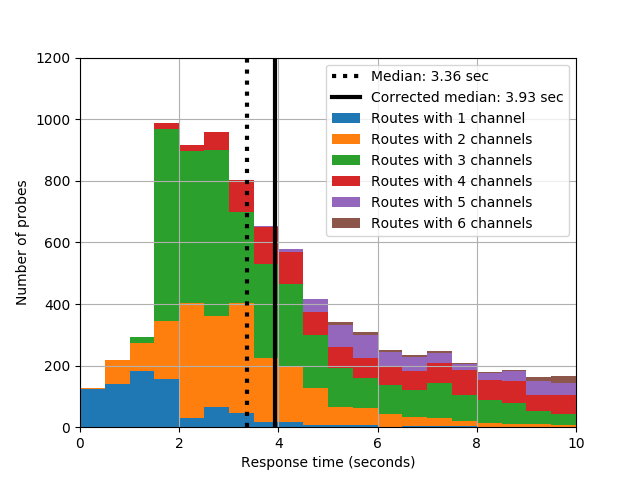
\includegraphics[width=0.8\textwidth]{route-length-timings.png}
	\caption{The distribution of probes (onions) by response time.}
	\label{fig:route-length-timings}
\end{figure}

Nearly all probes $3$~hops and shorter return within $10$~seconds.
The median of the $8\,256$~probes is at $3.36$~seconds.
Recall that $15.25\%$~of the probes timed out or returned an error that we could not interpret within out algorithm.
The corrected median without the timed out and erring probes is $3.93$~seconds. 
We conclude that the cutoff at $10$~seconds presents an acceptable trade-off.
The diameter of the strongly connected component on the LN is~$3$.\footnote{It is not always possible to use the shortest route, as it may not have sufficient balances in all channels.}

Next, we consider the time it takes to probe a single channel.
With the parameters we have chosen, each probe can not take longer than $70$~seconds ($7$~probes of up to $10$~seconds each).
For each channel, we add up the times of probes sent to this channel.
Figure~\ref{fig:channel-timings-CDF} shows the cumulative distribution function of channels by the total time spent probing them.
We observe that $50\%$~of channels can be probed in less than $21.2$~seconds.

\begin{figure}[ht]
	\centering
	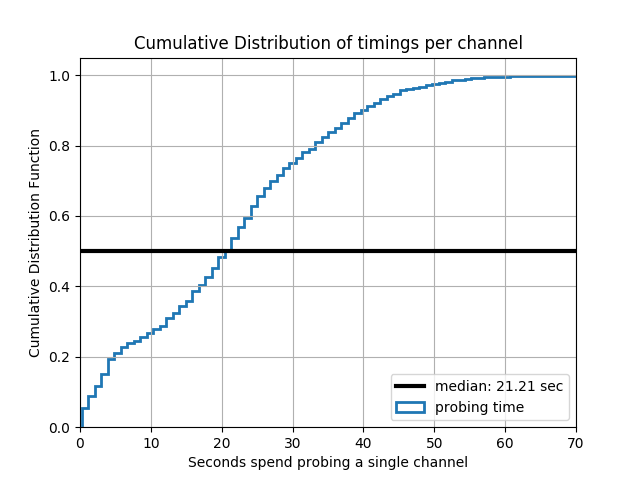
\includegraphics[width=0.8\textwidth]{channel-timings-CDF.png}
	\caption{Distribution of channels by total probing time.}
	\label{fig:channel-timings-CDF}
\end{figure}


\subsection{Probing coefficients}

We used the channel information coefficient to measure how much information we obtained for each channel.
At the time of the experiment, the LN specifications limited the value of a single payment to $0.043$~BTC\@.
We denote channels with the capacity more than two times that (i.e.,~$2 \times 0.043 = 0.086$~BTC) as \textit{large channels}.
We call other channels \textit{small}.
All small channels can in principle be fully probed.
A large channel can only be fully probed, if the local balance at one of its endpoints is smaller than the maximum payment amount.

\begin{figure}[ht]
	\centering
	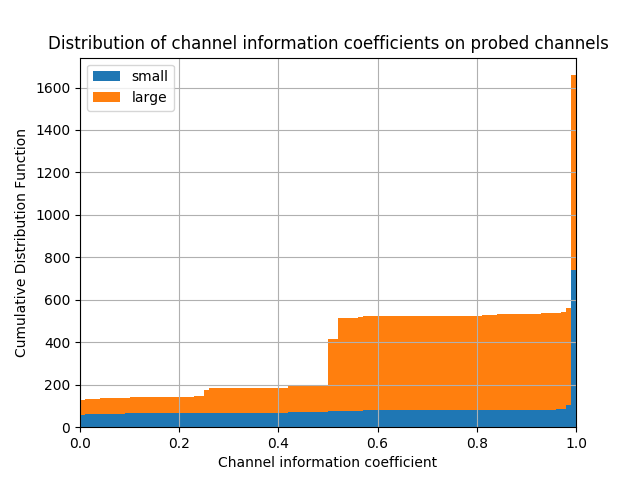
\includegraphics[width=0.8\textwidth]{cdf-channel-coefficients.png}
	\caption{Distribution of channels by the obtained information coefficient.}
	\label{fig:cdf-channel-coefficients}
\end{figure}

Figure~\ref{fig:cdf-channel-coefficients} represents the distribution of channels by their information coefficients.
We obtained full balance information on over $1\,000$ of~$1\,628$~channels.
Note that the jump at $0.5$~for the large channels is expected:the maximum standard channel capacity ($0.167$~BTC) is approximately four times the maximum HTLC amount ($0.043$).
Consider a channel with the total capacity of~$0.167$~BTC and the local balance between $0.043$~BTC and~$0.167 - 0.043 = 0.124$~BTC\@.
We probe this channel from both sides and receive the "unknown hash" error in both cases.
From that we conclude that the local balance is indeed between $0.043$~BTC and~$0.124$~BTC\@.
This estimate yields a channel information coefficient of~$0.515$.
However, with our current technique we cannot improve it.

\subsection{Distribution of channels in routes}

We also wanted to understand how often we send probes through each channel.
As Figure~\ref{fig:channel-frequency-distribution} shows, most of our routes go through the same few channels.
It is partially explained by all routes passing through one of our own entry channels.
%We suggest that this distribution, which seems to follow the power law, is consistent with the properties of a small world network with a small diameter.

\begin{figure}[h]
	\centering
	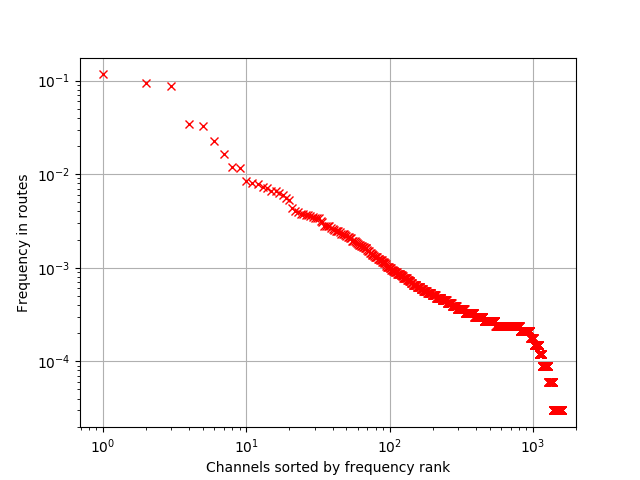
\includegraphics[width=0.8\textwidth]{channel-frequency-distribution.png}
	\caption{Distribution of relative frequencies of channels in routes.}
	\label{fig:channel-frequency-distribution}
\end{figure}


\subsection{How balanced are the channels?}

A Lightning channel is informally called \textit{balanced} if the parties have roughly equal balances.
We introduce the \textit{balance coefficient} to quantify this.
The balance coefficient represents the distance from the actual channel balance to $0.5$~of the total capacity, where $b$~is the estimated local balance and~$c$~is the total channel capacity:

\[c_{bal} = 0.5 - \frac{|b-c|}{c} \]

$c_{bal} = 0$~means the channel is unbalanced: the whole capacity is on one side.
$c_{bal} = 1$~means the channel is perfectly balanced: the two sides have equal balances.

\begin{figure}[h]
	\centering
	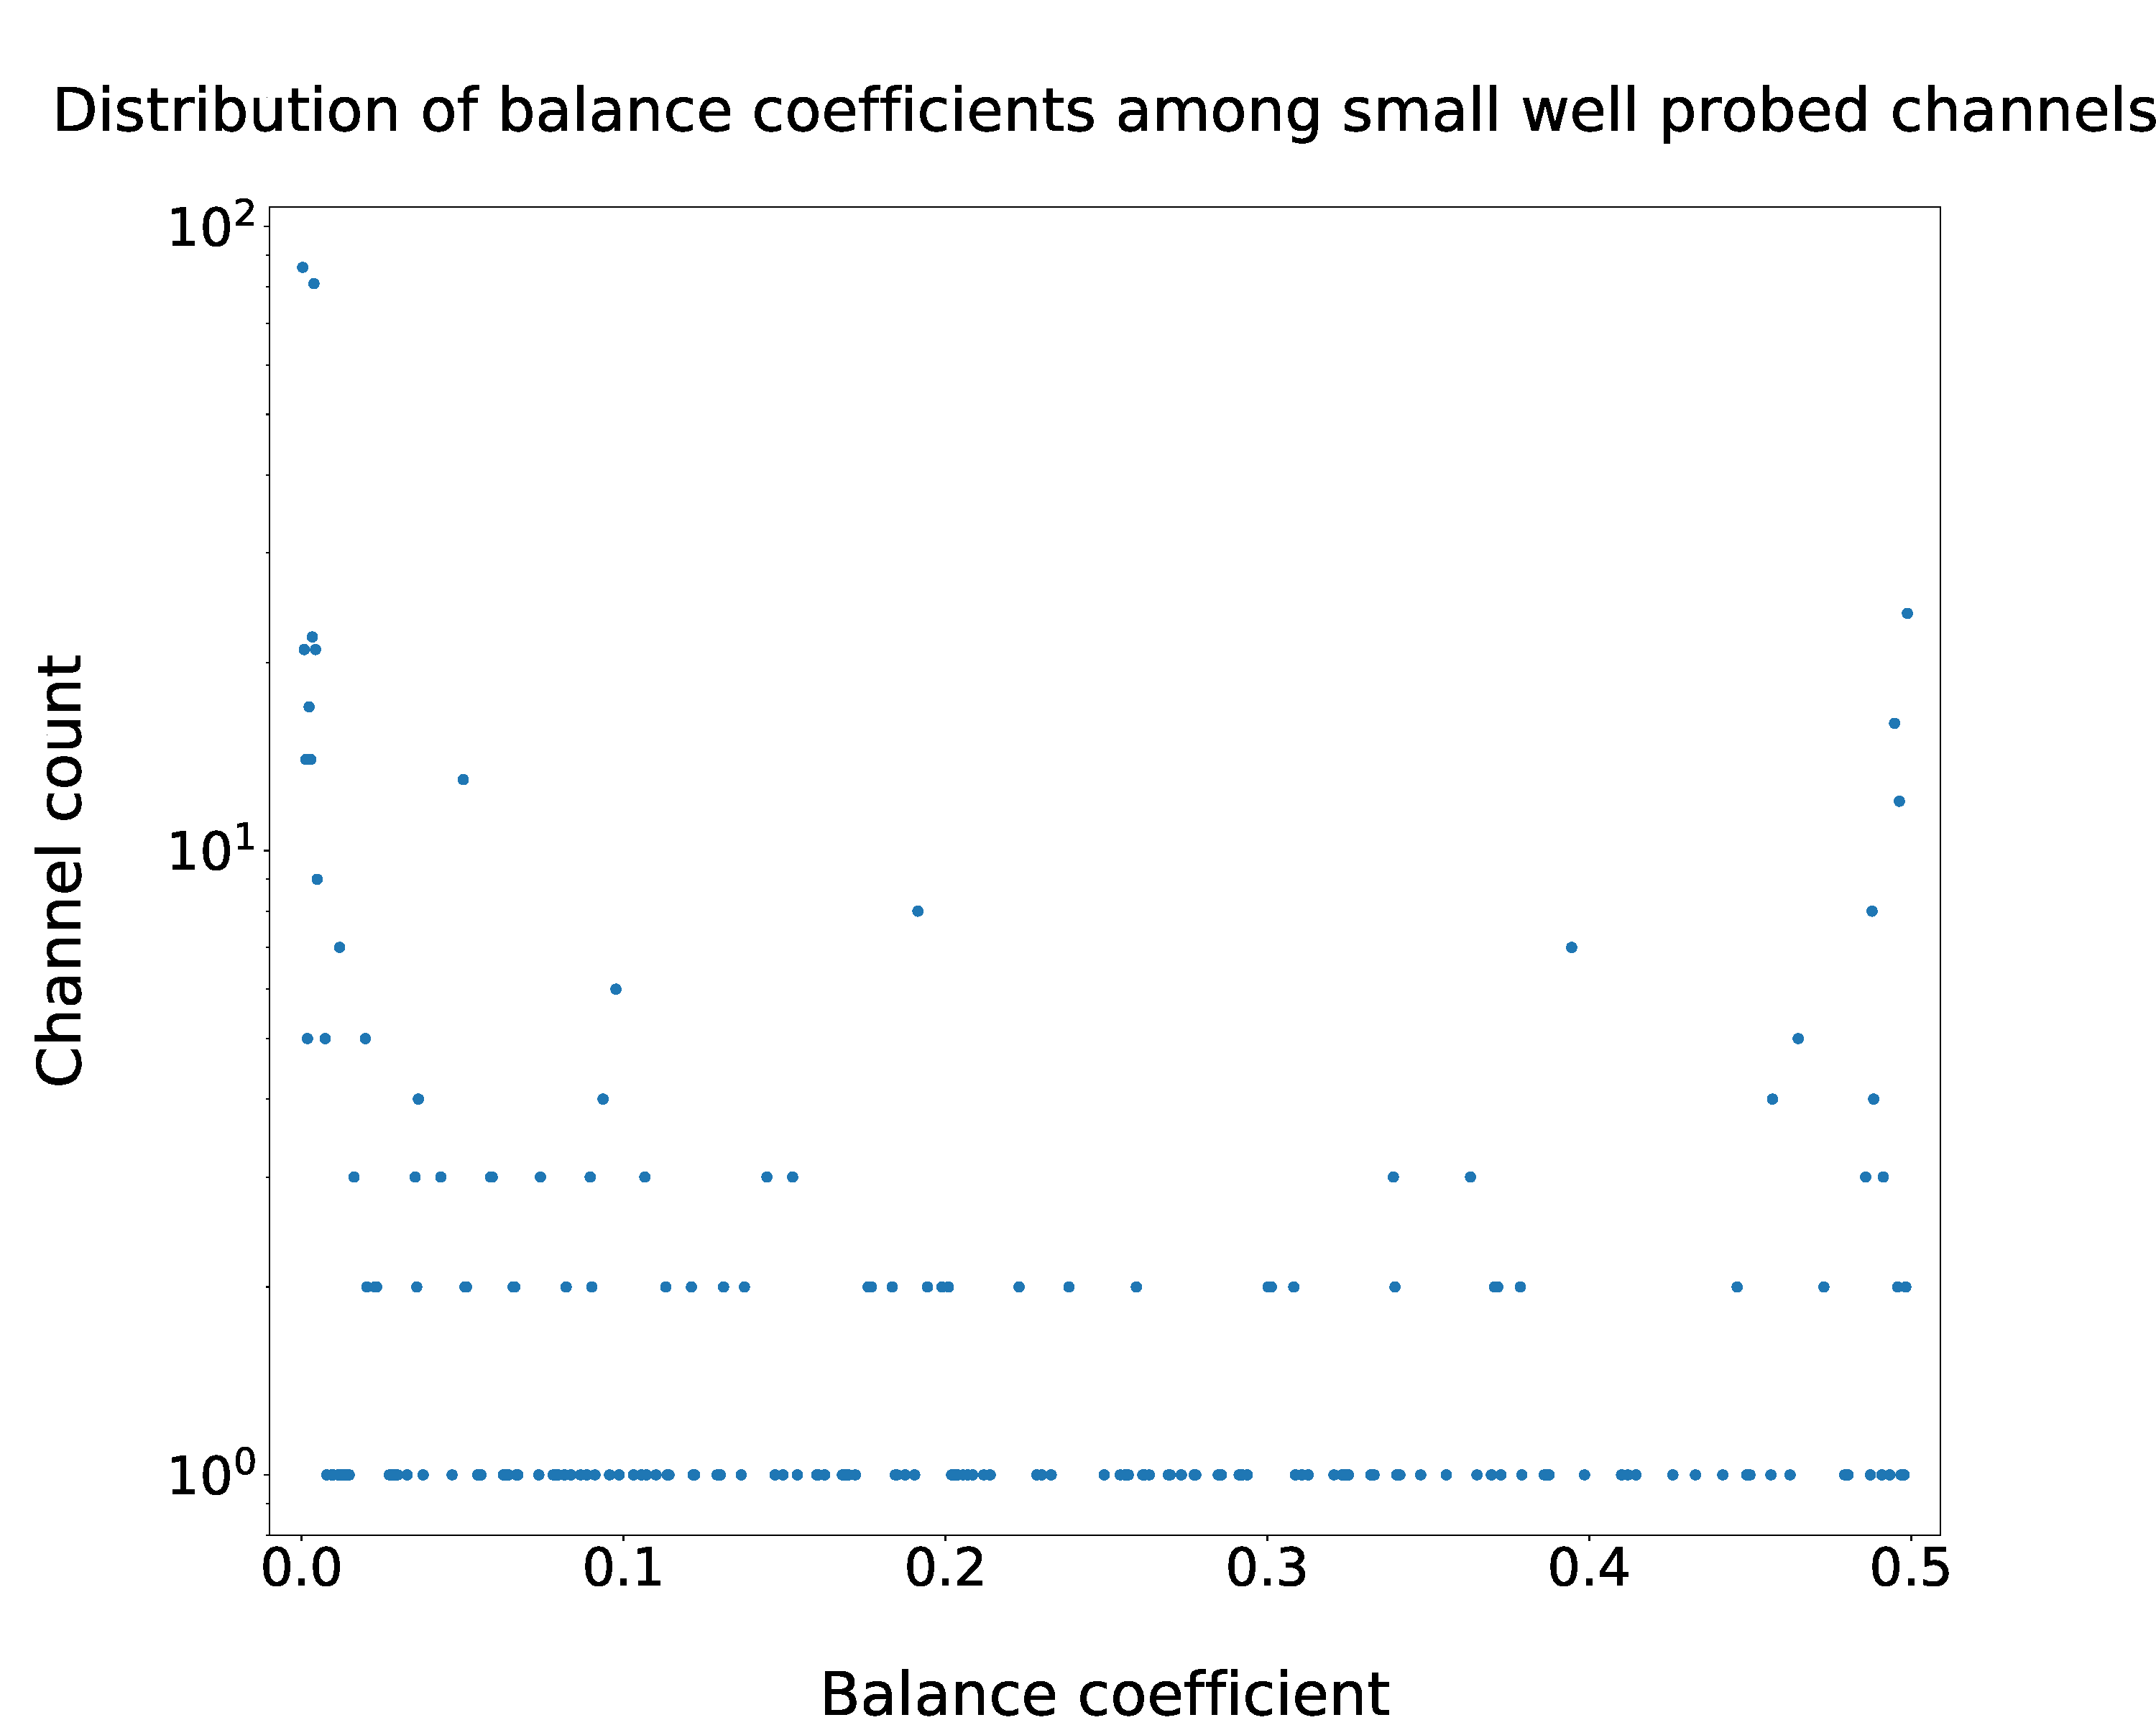
\includegraphics[width=0.8\textwidth]{balance-coeff-histogram.pdf}
	\caption{Distribution of balance coefficients.}
	\label{fig:balance-coeff-histogram}
\end{figure}

Figure~\ref{fig:balance-coeff-histogram} depicts the distribution of balance coefficients among "small" channels that we were able to probe with high accuracy (information coefficient higher than $0.9$).
We conclude that many small channels are unbalanced (coefficient close to zero).
$15\%$~have the balance coefficient below $0.001$, $45\%$~below $0.01$, and~$62\%$~below $0.1$.
Note, however, that the picture may change if we consider large channels, and that channel management practices on mainnet may differ significantly.


\section{Estimating the attack cost}

The attack requires moderate resources.
The attacker only needs to commit funds to the entry channels.
The capacities of the entry channels determine the maximum probe amount.
The computational and communication requirements are similar to the ones required to run a standard LN node.
The adversary only needs to maintain a few TCP connections during the main phase of the experiment.
(We also open and immediately close connections to all nodes to check their liveness; this process can be parallelized.)
Note that an LN node requires running a fully synchronized Bitcoin node, which requires hundreds of gigabytes of storage ($265$~GB at the time of our experiments in February~2020).

With our current approach, the maximum probing amount is the protocol's HTLC limit of~$0.167$~BTC\@.
This is the minimal amount the attacker has to commit to theoretically be able to fully probe all "small" channels.
Our experience shows that it is beneficial to open multiple channels to decrease the negative effect of hanging HTLCs.
In our experiments, we used five~entry channels.

Note that since all the probing transactions fail, the attacker pays no fees.
If no HLTCs are left unresolved after the probing, the attacker can close the entry channels collaboratively and withdraw the committed funds immediately.
If some HTLCs are left unresolved, or if the attacker's channel partners are offline or unwilling to cooperate on channel closure, the attacker would have to wait for the agreed upon timeout (usually on the order of days) before withdrawing the funds.
In any case, no coins committed to the attack are irrevocably lost.
However, the attacker still bears the opportunity cost: the bitcoins committed to the attack could have been invested elsewhere.


\section{Limitations}

Now we discuss the limitations of our approach and potential ways to improve it.

\paragraph{Private channels}

LN channels do not have to be announced.
For example, casual users using mobile devices are not supposed to announce their channels.
Such unannounced channels are called \textit{private}.
According to a 2020 study~\cite{BitMEXPrivateChannels}, $28\%$~of LN~channels are private.
Private channels are not prone to our probing methodology.
The sender does not know the identifier of the private channel party and cannot construct a route to it.

It may be possible to extend our technique with on-chain heuristics to locate private channel.
In particular, each channel has a short identifier composed of the number of the block, the transaction, and the UTXO index of the funding transaction.
An attacker may scan the blockchain looking for such outputs and cross-reference them with the LN gossip~\cite{Pickhardt2020}.

\paragraph{Lack of suitable routes}

We can not probe a route if we do not find a suitable route to the target channel.
In particular, we can not probe a high-capacity channel if it is connected to the rest of the network only through a low-capacity channel.
This limitation can be partially overcome by diverging from the series of probing amounts determined by binary search.
Recall that for each yet unknown channel balance $b$~we maintain the current estimation interval $[b_{min}, b_{max}]$.
The binary search prescribed to choose the next probing amount as $\frac{b_{min} + b_{max}}{2}$.
If this value is too high, we may choose the maximum value for which we can find a suitable route.
This would allow us to obtain at least some information on the channel in question.
In the initial version of our algorithm, we did not do it for simplicity.

\paragraph{Concurrent probing of large channels}

Recall that our method cannot fully probe large channels.
The reason behind this are the limitation on the HTLC amount.
Lightning implementations impose a limit on the maximal amount transferred in one HTLC\@.
This limit is approximately $0.043$~BTC\footnote{4294967295 millisatoshis.}.
Therefore, we can only fully probe channels where the local balance of one of the channel parties is below $0.043$~BTC\@.

A possible way to overcome this limitation would be to probe large channels with multiple HTLCs concurrently.
The goal of concurrent probing is to temporarily block the capacity of the attacked channel.
Our current method does not allow this, because we only control the sender, but not the receiver.
An honest receiver quickly returns an error, and the capacity is unblocked.
Therefore, concurrent probing would have to involve a malicious node acting as the receiver of all our probes.
It would deliberately delay the response, thus temporarily blocking funds along the route.

Concurrent probing could also decrease the probing time, bringing the results closer to an instant network snapshot.
However, adding concurrency is a non-trivial task.
Parallel probings may interfere with each other if the same channel is involved in two routes being probed at the same time.

Note also that certain realistic attack scenarios do not involve probing the whole network.
An adversary may choose one "important" Lightning node and probe all its channels relatively quickly.
The obtained information may be a business secret of the hub operator.


\paragraph{Parallel channels and non-strict forwarding}

Our method is based on an assumption that the probe is forwarded through the \textit{channels} determined by the sender.
However, the LN specification only guarantees that the sequence of \textit{nodes} is followed.
The channels shared by the same pair of nodes are referred to as \textit{parallel channels}.
A forwarding node is free to choose a channel from all parallel channel to the next node in the route.
This practice is known as \textit{non-strict forwarding} and provides flexibility in addressing local balance restrictions.
Therefore, we can not ensure that a probe is forwarded through a given channel.
It may be forwarded through a parallel channel instead.
This is true for all channels along the route.
We accept this as a limitation of our approach.

As seen from our LN snapshot dated 25~February~2020, the mainnet LN contained $1\,438$~parallel channels ($17.64\%$~of all channels), which indicates that the effects on the probing precision could be significant on mainnet\footnote{There may be private parallel channels, we can not estimate their effect on our results.}.
However, most \textit{node pairs} have no more than one channel, and can be probed using our method.
Note also that while the LN specification allows non-strict forwarding, the c-lightning implementation that we use does not support opening multiple channels to the same node.
The other two popular implementations, LND and Eclair, allow parallel channels.


\section{Countermeasures}
%\label{sec:discussion}

The simplest countermeasure that does not require protocol changes can be implemented as part of a node routing policy.
Note that all our payments used for probing fail (either due to insufficient balance or due to intentionally wrong hash value). 
Intermediary nodes know if a payment they are a part of succeeds or fails.
Therefore, an intermediary node observing a flood of failing payments from the same channel may assume that this is a probing, especially if the amounts follow the binary search pattern.
An intermediary node can then close the channel or otherwise limit the flow of failing payments from the node in question.
Of course, such techniques can be tricked.
An adversary can connect to Bob via Alice and make Bob think that Alice is performing the probing.

We divide the other potential countermeasures into two categories: those that prioritize privacy and those that prioritize efficiency.


\subsubsection*{Prioritizing privacy}

We argue that it is infeasible to reliably protect channel balances in the current LN protocol.
This conclusion comes from the following observations:
\begin{itemize}
	\item the sender knows whether the payment has failed or succeeded;
	\item if the payment has failed, the sender knows, which channel has failed.
\end{itemize}
However, we can change the protocol to make the latter assumption to not hold.

\paragraph{Merging error types}
When a payment fails, the sender receives an error message.
Depending on the cause of the error, these messages differ in two ways.
They have different error codes and originate from different nodes.
In particular, if the target channel has insufficient capacity, the error is returned by the \textit{previous} node.
If the target channel has enough capacity, then the \textit{final recipient} reports incorrect payment details.
We propose a change to LN error handling to prevent the sender from knowing where the payment has failed.
In particular, each node in a route changes the error it sends back as if it has originated from its own channel.
We also suggest merging the two error types ("incorrect or unknown payment details" and "temporary channel failure").
A similar countermeasure has already been implemented (see note about error types $16$~and~$17$~in BOLT4~\cite{Bolt4OnionRouting}).
The drawback of this method is a decrease in payment reliability.
The failing channel can no longer be excluded from the subsequent route search.
However, the payment reliability problem may become less pressing with \textit{multi-part payments} (MPP).
An MPP splits a large payment into smaller parts and increases routing flexibility.

\paragraph{Added loops}
Another potential countermeasure would be for intermediary nodes to add extra hops to the route.
Currently, the LN is source-routed: the route is chosen by the sender and enforced with onion routing.
Intermediary nodes can not change the sequence of nodes that a payment goes through (though they can choose a channel to the next node, if multiple channels are available).
If this scheme is modified, an intermediary node Alice could instead forward the payment to the next node in the route through an added random sub-route.
This would blur the picture for the sender, as the sender wouldn't know which path the payment has taken.
One drawback of this approach is the requirement to substantially change the onion routing protocol, which, as~\cite{Malavolta2019} argues, is necessary for LN security.
The fee structure would also have to be more complex.

\paragraph{JIT routing}
Just In Time Routing (JIT-routing) algorithm was originally proposed to improve payment reliability~\cite{Pickhardt2019, Pickhardt2019a}.
JIT routing works as follows.
If a forwarding node lacks the balance to forward a payment, it sends a circular payment to itself to add more funds to the required channel.
This process is called \textit{channel rebalancing}.\footnote{Another research paper~\cite{Conoscenti2019} analyzed the influence of hubs on LN and proposed a channel rebalancing algorithm.}
In the probing scenario, a JIT-supporting node does not send an error message back if it is lacking funds on the attacked (probed) channel.
Rather, it interrupts the routing process, re-balances its channels, and continue forwarding the payment.
The attacker would interpret this as a signal that the target channel has enough funds.
The same would hold if the channel is probed from the other side.
JIT routing can be an effective countermeasure against channel probing attacks.
However, as it takes more time, timing attacks may be possible. 


\subsubsection*{Prioritizing efficiency: sharing balance data}

If we conclude that it is infeasible to protect channel balances, we may want to use this information to improve routing efficiency.
Broadcasting all intermediate balances to all nodes is unfeasible, as it would introduce a large networking overhead.
% and structurally replicate the layer one (Bitcoin) gossip, where each transaction must reach every node.
%This puts severe limitations on layer one scalability, which is the problem LN is meant to solve.
We propose to develop a reasonable method for nodes to selectively share information about their channel balances.
This information would improve path-finding and help nodes decide how to allocate funds to new channels.
We propose adding an API call that would allow the sender to query the balance of a channel it wants to route a payment through.
In this scenario, a sender creates a preliminary route and asks the nodes along this route whether they have sufficient balance.
If some of them do not, the sender re-calculates the route until a suitable route is found.
This would improve upon the current LN payment workflow, where a sender is receiving errors and re-sending a payment along multiple routes until it succeeds.
Nodes could come up with policies regarding balances, for instance, only reveal balances to trusted nodes, or only to nodes that pay a fee.
The ability of a node to reveal a channel balance for routing purposes may also be subject to negotiation between channel partners during channel establishment.
We should also carry out a detailed analysis of ways to prevent abuse of this system.


\section{Conclusion} \label{sec:conclusion}

Hiding balances from everyone except for the channel parties is a cornerstone of L2 privacy.
Making intermediate channel balances available would enable revealing remote channel balances in real time.
However, unknown local balances negatively affect routing efficiency.
The sender cannot know in advance whether the chosen route can handle the required amount.
Therefore, LN payments often fail due to insufficient balance at an intermediary hop.
In that case, the payment is attempted again with a different route.
Knowing channel balances in advance could prevent such failures.

Our experiments show that channel balances can not be considered private data.
A low-resource attacker can probe the balances of most live and active channels with a high precision.
We implement and evaluate our technique on the Bitcoin testnet, successfully probing a large portion of channels.
We identify a \textit{privacy-efficiency trade-off}: hidden balances improve privacy but hinder routing efficiency.
LN does not address this trade-off optimally: channel balances are neither well protected nor utilized.
We envision two paths for LN development with either privacy or routing efficiency prioritized, and describe multiple directions for future work that would evaluate the ways to find the right balance between the two.